\documentclass[11pt,a4paper]{report}
\usepackage[utf8]{inputenc}
\usepackage[T1]{fontenc}
\usepackage{lmodern}
\usepackage{amsmath, amsthm, amssymb, amsfonts, enumitem}
\usepackage{graphicx}
\usepackage{dsfont}
\usepackage{mathtools}
\usepackage{pgfplots}
\pgfplotsset{compat=1.18}
\usepgfplotslibrary{groupplots,statistics}
\usepackage{xcolor}
\usepackage[colorlinks=true, linkcolor=blue, urlcolor=blue, citecolor=blue]{hyperref}
\usepackage{physics}

% Same macros as the paper, so equations and figures can be copied across.
\DeclareMathOperator{\spec}{spec}
\newcommand{\ot}{\otimes}
\newcommand{\one}{\mathds{1}}
\newcommand{\I}{\one}
\renewcommand{\a}{\alpha}
\renewcommand{\b}{\beta}
\newcommand{\N}{\mathds{N}}
\newcommand{\C}{\mathds{C}}
\newcommand{\cdk}{(\C^d)^{\otimes k}}

\newtheorem{theorem}{Theorem}[chapter]
\newtheorem{lemma}[theorem]{Lemma}
\newtheorem{result}[theorem]{Result}
\newtheorem{observation}[theorem]{Observation}
\theoremstyle{definition}
\newtheorem{definition}[theorem]{Definition}
\newtheorem{example}[theorem]{Example}

% Writing guidance. Delete every \note{...} before handing in;
% set \notesfalse to hide them all at once.
\newif\ifnotes \notestrue
\newcommand{\note}[1]{\ifnotes\par\medskip\noindent\fcolorbox{gray!60}{gray!8}{\parbox{\dimexpr\linewidth-2\fboxsep-2\fboxrule}{\small\textbf{To write.} #1}}\par\medskip\fi}

\begin{document}

% =====================================================================
\begin{titlepage}
\centering
{\large Master's internship report\par}
\vspace{1.5cm}
{\LARGE\bfseries Entanglement measures and LOCC conversion criteria\\ from Schur--Weyl duality\par}
\vspace{1.5cm}
{\Large Anton van Cleemput\par}
\vspace{1cm}
Master's programme: \textcolor{red}{[programme, university]}\par
Host laboratory: \textcolor{red}{[lab, institution]}\par
Supervisors: \textcolor{red}{[names]}\par
Internship period: \textcolor{red}{[start]} -- \textcolor{red}{[end]} 2026\par
\vfill
{\large \today\par}
\end{titlepage}

% =====================================================================
\begin{abstract}
\note{Write this last. About 150--250 words: the problem (quantifying entanglement and LOCC convertibility of mixed states), the approach (SDP hierarchy over entanglement spectra via Schur--Weyl duality), what you obtained (convergent bounds for any measure, Schmidt-number certificates, LOCC non-convertibility certificates, upper bounds from extracted decompositions), and the outputs of the internship (the arXiv preprint~\cite{ourPaper} and the two published libraries~\cite{boundEntangled,schurWeyl}).}
\end{abstract}

\chapter*{Acknowledgements}
\note{Supervisors, co-authors, the people thanked in the paper (Sophia Denker, Kenneth Goodenough, Ladina Hausmann, Renato Renner, Karol \.Zyczkowski), the host lab, and the funding. Keep the AI statement consistent with the paper's (see the end of the conclusion chapter).}

\tableofcontents

% =====================================================================
\chapter{Introduction}\label{ch:intro}

\section{Context}
\note{Why entanglement matters as a resource; pure states are fully understood through the entanglement spectrum (Nielsen~\cite{Nielsen1999MajLOCC}, Vidal~\cite{Vidal_1999,Vidal_2000}); mixed states need convex roofs, which are hard to compute~\cite{Bennett1996EoF,Uhlmann2010Roofs}. The paper's introduction is a good compressed version: expand it for a reader who is a physicist but not a quantum information specialist.}

\section{Goal of the internship}
\note{The question you started with in May (Schmidt number from isotypic projectors, see \texttt{material.md} \S1) and how it grew into the general method of the paper.}

\section{Contributions}
\note{A list. Separate clearly: (i) your own contributions, (ii) joint work with co-authors, (iii) the published outputs: the preprint~\cite{ourPaper}, \texttt{bound-entangled}~\cite{boundEntangled}, \texttt{schur-weyl}~\cite{schurWeyl}. Check the split with your supervisors (\texttt{material.md} \S2 and \S8).}

\section{Outline}
\note{One sentence per chapter.}

% =====================================================================
\chapter{Background}\label{ch:background}

\section{Entanglement, LOCC and the entanglement spectrum}
\note{Schmidt decomposition, Schmidt rank, Nielsen's majorization theorem~\cite{Nielsen1999MajLOCC}, Vidal monotones~\cite{Vidal_1999}, the Jonathan--Plenio criterion for pure-to-ensemble conversion~\cite{Jonathan_1999}. A worked two-qubit example helps.}

\section{Mixed states and convex roofs}
\note{Convex roof extension, entanglement of formation~\cite{Bennett1996EoF}, Wootters' formula for two qubits~\cite{Wootters1998} (which you use as ground truth), Schmidt number~\cite{Terhal_2000}, why the optimization is hard. The HJW / Schr\"odinger parametrisation of decompositions~\cite{schrodinger36,HJW}.}

\section{Semidefinite programming}
\note{Primal and dual, weak and strong duality, interior-point solvers. The symmetric-extension hierarchy for separability~\cite{doherty2002} as the closest known analogue of your hierarchy.}

\section{Symmetric polynomials and Schur--Weyl duality}
\note{Partitions and Young diagrams, the Schur--Weyl decomposition~\cite{fulton2013representation}, isotypic projectors, Schur polynomials and Kostka numbers~\cite{MacdonaldSymmFunc}, weak Schur sampling~\cite{Alicki1988,Keyl2001EstimatingSpectrum}. This is where the paper is most compressed, so it is the best place to show understanding. Small examples: $k=2$ (symmetric and antisymmetric subspaces), $k=3$ with $\lambda=(2,1)$.}

\section{Bound entangled states}
\note{What bound entanglement is, the families used in the experiments (Horodecki, chessboard, UPB-based states such as tiles and pyramid, Piani, \dots), and how your \texttt{bound-entangled} package collects them~\cite{boundEntangled}.}

% =====================================================================
\chapter{First phase: Schmidt number from isotypic projectors}\label{ch:phase1}
\note{May--September, project \texttt{QuantifyingSchmidtNumber} (\texttt{material.md} \S1). The SDP with a single isotypic projector as objective, the $E_t$ bounds, the state sweeps (convex mixtures, noise, parametric families), binary searches for thresholds, the Tavakoli and isotropic Schmidt-number-3 results, the cluster runs and the results viewer. Explain what you learned that led to the general method of Chapter~\ref{ch:method}. A figure from \texttt{sdp\_results/} would fit here.}

% =====================================================================
\chapter{Method}\label{ch:method}
\note{The paper's main text, with more intuition before each formal statement. Proofs can be summarised and referred to the preprint~\cite{ourPaper}; give at least one proof in full (for example the convergence of the hierarchy) to show you master it. The key equations are copied from the paper so that labels and figure captions work.}

\section{Polynomial measures as linear functionals}
\note{Schur basis, the observable $O_P$, the decomposition state $\omega_k=\sum_ip_i\dyad{\psi_i}^{\otimes k}$~\cite{Toth2015CroofTP}.}

\section{The SDP hierarchy}
\begin{align}
    P_{{\rm LB}_k}(\rho)=\min_{\Omega_k} \ &\tr\!\left(O_P^A \otimes \I^B \, \Omega_k\right)\label{eq:SDPcroof1}\\
    \text{s.t. } & \Omega_k \succeq 0, \nonumber\\
    & \Pi_\text{sym}^{AB,k} \, \Omega_k = \Omega_k\,\Pi_\text{sym}^{AB,k}  = \Omega_k,\nonumber\\
    & \tr_{2,\dots,k} (\Omega_k) = \rho, \nonumber\\
    & \Omega_k^{T_l} \succeq 0 \quad  \forall \, l \in \{1, \dots, \lfloor \tfrac{k}{2}\rfloor\}.\nonumber
\end{align}
\note{Convergence via the de Finetti theorem~\cite{Christandl_2007} and continuity of the convex roof~\cite{Bucicovschi2013}; monotonicity in $k$; the Schmidt-number certificate and the example of Ref.~\cite{Tavakoli_2024}.}

\section{The simplified relaxation}
\begin{align}\label{eq:marginals_SDP}
    P_{{\rm LB}_{k,m}}:=&\min_{\Phi_{k,m}} \tr(O_P^A \otimes \I^B \ \Phi_{k,m})\\
    \text{s.t. } & \Phi_{k,m}\succeq 0, \nonumber\\
    & \Pi_\text{sym}^{AB,k} \, \Phi_{k}\, \Pi_\text{sym}^{AB,k}= \Phi_{k},\nonumber\\
    & \tr_{A_2,\dots,A_m,B_2,\dots,B_k} (\Phi_{k,m}) = \rho_{AB}, \nonumber\\
    & \tr_{B_1,\dots,B_k}(\Phi_{k,m}) \text{ is permutation invariant},\nonumber\\
    & \Phi_{k,m}^{T_S} \succeq 0 \quad  \forall \, S.\nonumber
\end{align}
\note{Why it is cheaper for full-rank states; the trade-off is quantified in Chapter~\ref{ch:implementation}.}

\section{Upper bounds from the SDP solution}
\note{Extraction: rank reduction, Jennrich~\cite{Harshman1970,Leurgans1993}, PARAFAC~\cite{CarrollChang1970,tensorly}, the repair step $\rho^{1/2}\sigma^{-1/2}$, uniqueness~\cite{Kruskal1977}. Gradient descent over HJW unitaries~\cite{HJW,Rothlisberger2009} as the comparison. The tightness certificate (\texttt{material.md} \S4).}

\section{Non-polynomial measures}
\note{The grid, the LP and its dual, merging into one SDP, the grid error, convergence (Weierstrass). Figure~\ref{fig:grid} explains the grid. The comparison of polynomial classes (A, B, C) is in \texttt{material.md} \S4 and is not in the paper.}

\begin{figure}[t]
    \centering
    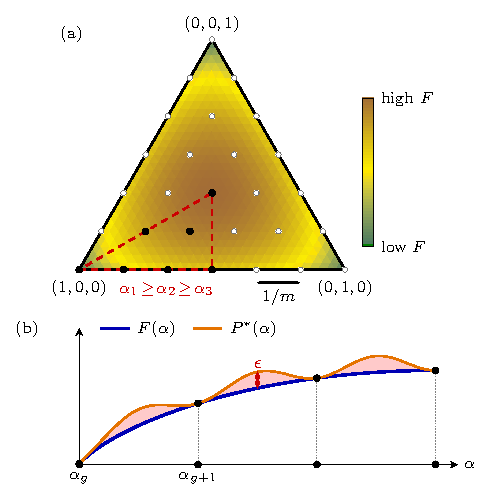
\includegraphics{figures/grid_simplex}
    \caption{Grid discretization of the simplex of spectra for $d_A=3$.
    (a) Different values of $F(\alpha)$ are denoted by different colors. The dots denote the grid $G$, separated by a certain distance $1/m$. Since entanglement measures are symmetric functions on the spectrum, only the points with $\alpha_1\geq\alpha_2\geq\alpha_3$ (dashed region, filled dots) need to be imposed.
    (b) Cut along a one-parameter family of spectra. Although $P^*\leq F$ holds at all grid points, it is possible that $P^*>F$ between any two points by a value $\epsilon$. This value decreases as we refine the grid.}
    \label{fig:grid}
\end{figure}

\section{LOCC convertibility}
\begin{align}\label{eq:LOCCminmaxt}
    s_k=\min_{\Omega_k} \max_t \max_{P_j\in\mathcal{P}_j}\ \sum_j t_j\Big(\tr\left((O_{P_j}\otimes\I^B)\Omega_k\right)-E_j(\psi)\Big),
\end{align}
\note{Joint constraints for all Vidal monotones, the certificate of non-convertibility, the heuristic for convertibility by extraction, and why extraction can fail here.}

% =====================================================================
\chapter{Implementation}\label{ch:implementation}
\note{The chapter where most of your internship time shows. Use \texttt{material.md} \S3.}

\section{Software architecture}
\note{Layout of \texttt{src/} and \texttt{experiments/}, the test suite with brute-force cross-checks, resumable result files, the figure pipeline (scripts $\to$ CSV $\to$ pgfplots). A diagram would help.}

\section{Symmetry reductions}
\note{Symmetric subspace, bosonic operators for the marginal constraint, partial transposes on $\mathrm{Sym}^l\otimes\mathrm{Sym}^{k-l}$, projection on the support of $\rho$, real variables (paper App.~D). Add the caveat that a real $\rho$ does not imply a real optimal decomposition.}

\section{Solvers and numerical issues}
\note{From picos to a native sparse QICS model~\cite{qics} (memory 15\,GB $\to$ 3\,GB); the pitfalls you hit and how you fixed them (\texttt{material.md} \S3).}

\section{Memory cost}
\note{The variable-count formula, the $8n^2$ model, the rule $r<(k+1)r_A-k$, the measurement pitfall you caught, and Fig.~\ref{fig:memory}.}
% Shared colors and styles of the figures. Every figure reads its data from figures/data/*.csv, written by
% experiments/make_figures.py (comma separated, header row, nan for missing values: pgfplots skips those points).
\definecolor{cA}{HTML}{2a78d6}\definecolor{cB}{HTML}{eb6834}\definecolor{cC}{HTML}{1baf7a}%
\definecolor{cD}{HTML}{4a3aa7}\definecolor{cE}{HTML}{c03b7a}\definecolor{cF}{HTML}{8a6d1f}\definecolor{cGray}{HTML}{8a8984}%
\definecolor{lvA}{HTML}{c6dbf5}\definecolor{lvB}{HTML}{93bbec}\definecolor{lvC}{HTML}{5e98e0}%
\definecolor{lvD}{HTML}{2a78d6}\definecolor{lvE}{HTML}{174a8c}\definecolor{lvF}{HTML}{1baf7a}%
%
% \namedbars{csv file}{ylabel}{title}: lower bounds of the named states at every level, divided by the reference `ref`
% (printed above each state at height `label_y`), with the two upper bounds as markers. Columns: see named_csv in
% make_figures.py. The state positions (`pos`) leave a gap at x = 10 between the PPT and the NPT states.
\providecommand{\namedbar}[3]{% fill, column, offset
  \addplot[ybar, bar width=0.13, bar shift=0pt, draw=none, fill=#1, area legend]
    table[x expr=\thisrow{pos}+#3, y expr=\thisrow{#2}/\thisrow{ref}] {\namedfile};}
\providecommand{\namedbars}[3]{%
  \def\namedfile{#1}%
  \begin{tikzpicture}
    \begin{axis}[width=\textwidth, height=0.29\textwidth, ymin=0, ymax=1.38, xmin=0.3, xmax=14.7,
      ylabel={#2}, ytick={0,0.25,0.5,0.75,1}, xtick=data, xticklabels from table={#1}{state},
      table/col sep=comma, xticklabel style={rotate=35, anchor=north east, font=\scriptsize, inner sep=1pt},
      tick label style={font=\footnotesize}, label style={font=\small}, title={#3}, title style={font=\small,
      yshift=8pt}, clip=false, legend style={font=\scriptsize, at={(0.5,-0.42)}, anchor=north, legend columns=4,
      draw=none, /tikz/every even column/.append style={column sep=6pt}}, legend cell align=left,
      ytick style={draw=none}, xtick style={draw=none}, ymajorgrids, grid style={cGray!25}]
      \addplot[draw=none, forget plot] table[x=pos, y expr=0] {#1};% the ticks (xtick=data)
      \namedbar{lvA}{lb12}{-0.325}\addlegendentry{LB $(1,2)$}
      \namedbar{lvB}{lb13}{-0.195}\addlegendentry{LB $(1,3)$}
      \namedbar{lvC}{lb22}{-0.065}\addlegendentry{LB $(2,2)$}
      \namedbar{lvD}{lb23}{0.065}\addlegendentry{LB $(2,3)$}
      \namedbar{lvE}{lb33}{0.195}\addlegendentry{LB $(3,3)$}
      \namedbar{lvF}{lb24}{0.325}\addlegendentry{LB $(2,4)$}
      \addplot[only marks, mark=diamond*, mark size=2.2pt, cB, mark options={draw=white, line width=0.4pt}]
        table[x expr=\thisrow{pos}-0.14, y expr=\thisrow{ub_extract}/\thisrow{ref}] {#1};
      \addlegendentry{UB: extracted ($k=m=3$)}
      \addplot[only marks, mark=x, mark size=2.4pt, black, thick]
        table[x expr=\thisrow{pos}+0.14, y expr=\thisrow{ub_hjw}/\thisrow{ref}] {#1};
      \addlegendentry{UB: HJW}
      \addplot[only marks, mark=none, nodes near coords={$\pgfplotspointmeta$}, point meta=explicit symbolic,
        nodes near coords style={anchor=south, font=\tiny, inner sep=1pt}, forget plot]
        table[x=pos, y=label_y, meta=ref_label] {#1};
      \draw[cGray] (axis cs:0.3,1) -- (axis cs:14.7,1);
      \draw[cGray, densely dashed] (axis cs:10,0) -- (axis cs:10,1.38);
      \node[font=\scriptsize, anchor=south] at (axis cs:5,1.38) {PPT (bound entangled)};
      \node[font=\scriptsize, anchor=south] at (axis cs:12.5,1.38) {NPT};
    \end{axis}
  \end{tikzpicture}}
%
% \memcurve{state}{color}{mark}{legend}: the measured memory of one state (column mem_<state> of memory.csv), broken
% between the groups of levels of equal degree m (pos 1-2: m = 2, pos 4-6: m = 3, pos 8-11: m = 4).
\providecommand{\memcurve}[4]{%
  \addplot[#2, thick, mark=#3, mark size=1pt, restrict x to domain=0:2.5] table[x=pos, y=mem_#1] {\memfile};
  \addlegendentry{#4}
  \addplot[#2, thick, mark=#3, mark size=1.8pt, restrict x to domain=3.5:6.5, forget plot]
    table[x=pos, y=mem_#1] {\memfile};
  \addplot[#2, thick, mark=#3, mark size=1.8pt, restrict x to domain=7.5:11.5, forget plot]
    table[x=pos, y=mem_#1] {\memfile};}%
\providecommand{\fulllevel}[1]{\fill[cGray!15] (axis cs:#1-0.4,0.01) rectangle (axis cs:#1+0.4,32);}%
\begin{figure}[htbp]
  \centering
  \def\memfile{figures/data/memory.csv}%
  \begin{tikzpicture}
    \begin{axis}[name=memaxis, width=0.7\textwidth, height=0.49\textwidth, ymode=log, ymin=0.01, ymax=32, xmin=0.4, xmax=11.6,
      xtick=data, xticklabels from table={figures/data/memory.csv}{level}, xlabel={level $(k,m)$},
      ytick={0.01,0.1,1,10}, yticklabels={10\,MB,100\,MB,1\,GB,10\,GB}, ylabel={memory},
      xticklabel style={rotate=45, anchor=north east, font=\scriptsize, inner sep=1pt},
      tick label style={font=\footnotesize}, label style={font=\small}, xtick style={draw=none},
      ymajorgrids, grid style={cGray!25}, clip=false, table/col sep=comma,
      legend to name=memlegend,
      legend style={font=\scriptsize, draw=none, legend columns=3,
      /tikz/every even column/.append style={column sep=4pt}}, legend cell align=left]
      \fulllevel{2}\fulllevel{6}\fulllevel{11}
      \addplot[draw=none, forget plot] table[x=pos, y expr=1] {\memfile};% the ticks (xtick=data)
      \memcurve{r4a2}{cA}{*}{$r=4$, $r_A=2$}
      \memcurve{r4a3}{cB}{square*}{$r=4$, $r_A=3$}
      \memcurve{r9a3}{cC}{triangle*}{$r=9$, $r_A=3$}
      \memcurve{r4a4}{cD}{diamond*}{$r=4$, $r_A=4$}
      \memcurve{r8a4}{cE}{pentagon*}{$r=8$, $r_A=4$}
      \memcurve{r16a4}{cF}{star}{$r=16$, $r_A=4$}      \node[font=\scriptsize, anchor=south] at (axis cs:1.5,32) {$m=2$};
      \node[font=\scriptsize, anchor=south] at (axis cs:5,32) {$m=3$};
      \node[font=\scriptsize, anchor=south] at (axis cs:9.5,32) {$m=4$};
    \end{axis}
    \node[anchor=north, yshift=-2pt] at (memaxis.outer south) {\pgfplotslegendfromname{memlegend}};
  \end{tikzpicture}
  \caption{Memory needed by the SDP~\eqref{eq:marginals_SDP} with the QICS solver~\cite{qics} at different levels for random states $\rho$ with $r=\operatorname{rank}(\rho)$ and $r_A = \operatorname{rank}(\tr_B(\rho))$. When $k=m$, the full SDP~\eqref{eq:SDPcroof1} is used.}
  \label{fig:memory}
\end{figure}


\section{Libraries}
\note{\texttt{bound-entangled}~\cite{boundEntangled} and \texttt{schur-weyl}~\cite{schurWeyl}: why you wrote them, design choices (numpy only, tests, documentation sites, PyPI publishing workflow), and how the main code uses them.}

% =====================================================================
\chapter{Results}\label{ch:results}
\note{The paper's figures with more discussion of each, plus results not in the paper (\texttt{material.md} \S4). Say for each figure what the reader should take away.}

\section{Linear entropy}
% Shared colors and styles of the figures. Every figure reads its data from figures/data/*.csv, written by
% experiments/make_figures.py (comma separated, header row, nan for missing values: pgfplots skips those points).
\definecolor{cA}{HTML}{2a78d6}\definecolor{cB}{HTML}{eb6834}\definecolor{cC}{HTML}{1baf7a}%
\definecolor{cD}{HTML}{4a3aa7}\definecolor{cE}{HTML}{c03b7a}\definecolor{cF}{HTML}{8a6d1f}\definecolor{cGray}{HTML}{8a8984}%
\definecolor{lvA}{HTML}{c6dbf5}\definecolor{lvB}{HTML}{93bbec}\definecolor{lvC}{HTML}{5e98e0}%
\definecolor{lvD}{HTML}{2a78d6}\definecolor{lvE}{HTML}{174a8c}\definecolor{lvF}{HTML}{1baf7a}%
%
% \namedbars{csv file}{ylabel}{title}: lower bounds of the named states at every level, divided by the reference `ref`
% (printed above each state at height `label_y`), with the two upper bounds as markers. Columns: see named_csv in
% make_figures.py. The state positions (`pos`) leave a gap at x = 10 between the PPT and the NPT states.
\providecommand{\namedbar}[3]{% fill, column, offset
  \addplot[ybar, bar width=0.13, bar shift=0pt, draw=none, fill=#1, area legend]
    table[x expr=\thisrow{pos}+#3, y expr=\thisrow{#2}/\thisrow{ref}] {\namedfile};}
\providecommand{\namedbars}[3]{%
  \def\namedfile{#1}%
  \begin{tikzpicture}
    \begin{axis}[width=\textwidth, height=0.29\textwidth, ymin=0, ymax=1.38, xmin=0.3, xmax=14.7,
      ylabel={#2}, ytick={0,0.25,0.5,0.75,1}, xtick=data, xticklabels from table={#1}{state},
      table/col sep=comma, xticklabel style={rotate=35, anchor=north east, font=\scriptsize, inner sep=1pt},
      tick label style={font=\footnotesize}, label style={font=\small}, title={#3}, title style={font=\small,
      yshift=8pt}, clip=false, legend style={font=\scriptsize, at={(0.5,-0.42)}, anchor=north, legend columns=4,
      draw=none, /tikz/every even column/.append style={column sep=6pt}}, legend cell align=left,
      ytick style={draw=none}, xtick style={draw=none}, ymajorgrids, grid style={cGray!25}]
      \addplot[draw=none, forget plot] table[x=pos, y expr=0] {#1};% the ticks (xtick=data)
      \namedbar{lvA}{lb12}{-0.325}\addlegendentry{LB $(1,2)$}
      \namedbar{lvB}{lb13}{-0.195}\addlegendentry{LB $(1,3)$}
      \namedbar{lvC}{lb22}{-0.065}\addlegendentry{LB $(2,2)$}
      \namedbar{lvD}{lb23}{0.065}\addlegendentry{LB $(2,3)$}
      \namedbar{lvE}{lb33}{0.195}\addlegendentry{LB $(3,3)$}
      \namedbar{lvF}{lb24}{0.325}\addlegendentry{LB $(2,4)$}
      \addplot[only marks, mark=diamond*, mark size=2.2pt, cB, mark options={draw=white, line width=0.4pt}]
        table[x expr=\thisrow{pos}-0.14, y expr=\thisrow{ub_extract}/\thisrow{ref}] {#1};
      \addlegendentry{UB: extracted ($k=m=3$)}
      \addplot[only marks, mark=x, mark size=2.4pt, black, thick]
        table[x expr=\thisrow{pos}+0.14, y expr=\thisrow{ub_hjw}/\thisrow{ref}] {#1};
      \addlegendentry{UB: HJW}
      \addplot[only marks, mark=none, nodes near coords={$\pgfplotspointmeta$}, point meta=explicit symbolic,
        nodes near coords style={anchor=south, font=\tiny, inner sep=1pt}, forget plot]
        table[x=pos, y=label_y, meta=ref_label] {#1};
      \draw[cGray] (axis cs:0.3,1) -- (axis cs:14.7,1);
      \draw[cGray, densely dashed] (axis cs:10,0) -- (axis cs:10,1.38);
      \node[font=\scriptsize, anchor=south] at (axis cs:5,1.38) {PPT (bound entangled)};
      \node[font=\scriptsize, anchor=south] at (axis cs:12.5,1.38) {NPT};
    \end{axis}
  \end{tikzpicture}}
%
\begin{figure}[htbp]
  \centering
  \begin{tikzpicture}
    \begin{axis}[width=0.6\textwidth, height=0.43\textwidth, xlabel={$a$}, ylabel={bounds on $\widehat{S_L}$},
      ymin=0, ymax=4.2e-3, scaled y ticks=base 10:3, tick label style={font=\footnotesize}, label style={font=\small},
      legend style={font=\scriptsize, at={(0.5,-0.24)}, anchor=north, draw=none, legend columns=3,
      /tikz/every even column/.append style={column sep=4pt}}, legend cell align=left, table/col sep=comma]
      \def\file{figures/data/linear_entropy_horodecki24.csv}
      \addplot[lvA, thick] table[x=a, y=lb12] {\file};\addlegendentry{LB $(1,2)$}
      \addplot[lvB, thick] table[x=a, y=lb13] {\file};\addlegendentry{LB $(1,3)$}
      \addplot[lvC, thick] table[x=a, y=lb22] {\file};\addlegendentry{LB $(2,2)$}
      \addplot[lvD, thick] table[x=a, y=lb23] {\file};\addlegendentry{LB $(2,3)$}
      \addplot[lvE, thick, densely dashed] table[x=a, y=lb33] {\file};\addlegendentry{LB $(3,3)$}
      \addplot[lvF, very thick, dotted] table[x=a, y=lb24] {\file};\addlegendentry{LB $(2,4)$}
      \addplot[only marks, mark=diamond, mark size=3pt, cB, thick] table[x=a, y=ub_extract] {\file};
      \addlegendentry{UB: extracted, $k=m=3$}
      \addplot[only marks, mark=x, black, thick, mark size=1.8pt] table[x=a, y=ub_hjw] {\file};\addlegendentry{UB: HJW}
    \end{axis}
  \end{tikzpicture}
  \caption{Convex roof of the linear entropy $S_L=1-\tr\rho_A^2$ for the Horodecki $2\times4$ family. Lower bounds are shown at different levels of the hierarchy. The markers show the upper bounds extracted from our method and HJW gradient descent.}
  \label{fig:linearEntropy}
\end{figure}

% Shared colors and styles of the figures. Every figure reads its data from figures/data/*.csv, written by
% experiments/make_figures.py (comma separated, header row, nan for missing values: pgfplots skips those points).
\definecolor{cA}{HTML}{2a78d6}\definecolor{cB}{HTML}{eb6834}\definecolor{cC}{HTML}{1baf7a}%
\definecolor{cD}{HTML}{4a3aa7}\definecolor{cE}{HTML}{c03b7a}\definecolor{cF}{HTML}{8a6d1f}\definecolor{cGray}{HTML}{8a8984}%
\definecolor{lvA}{HTML}{c6dbf5}\definecolor{lvB}{HTML}{93bbec}\definecolor{lvC}{HTML}{5e98e0}%
\definecolor{lvD}{HTML}{2a78d6}\definecolor{lvE}{HTML}{174a8c}\definecolor{lvF}{HTML}{1baf7a}%
%
% \namedbars{csv file}{ylabel}{title}: lower bounds of the named states at every level, divided by the reference `ref`
% (printed above each state at height `label_y`), with the two upper bounds as markers. Columns: see named_csv in
% make_figures.py. The state positions (`pos`) leave a gap at x = 10 between the PPT and the NPT states.
\providecommand{\namedbar}[3]{% fill, column, offset
  \addplot[ybar, bar width=0.13, bar shift=0pt, draw=none, fill=#1, area legend]
    table[x expr=\thisrow{pos}+#3, y expr=\thisrow{#2}/\thisrow{ref}] {\namedfile};}
\providecommand{\namedbars}[3]{%
  \def\namedfile{#1}%
  \begin{tikzpicture}
    \begin{axis}[width=\textwidth, height=0.29\textwidth, ymin=0, ymax=1.38, xmin=0.3, xmax=14.7,
      ylabel={#2}, ytick={0,0.25,0.5,0.75,1}, xtick=data, xticklabels from table={#1}{state},
      table/col sep=comma, xticklabel style={rotate=35, anchor=north east, font=\scriptsize, inner sep=1pt},
      tick label style={font=\footnotesize}, label style={font=\small}, title={#3}, title style={font=\small,
      yshift=8pt}, clip=false, legend style={font=\scriptsize, at={(0.5,-0.42)}, anchor=north, legend columns=4,
      draw=none, /tikz/every even column/.append style={column sep=6pt}}, legend cell align=left,
      ytick style={draw=none}, xtick style={draw=none}, ymajorgrids, grid style={cGray!25}]
      \addplot[draw=none, forget plot] table[x=pos, y expr=0] {#1};% the ticks (xtick=data)
      \namedbar{lvA}{lb12}{-0.325}\addlegendentry{LB $(1,2)$}
      \namedbar{lvB}{lb13}{-0.195}\addlegendentry{LB $(1,3)$}
      \namedbar{lvC}{lb22}{-0.065}\addlegendentry{LB $(2,2)$}
      \namedbar{lvD}{lb23}{0.065}\addlegendentry{LB $(2,3)$}
      \namedbar{lvE}{lb33}{0.195}\addlegendentry{LB $(3,3)$}
      \namedbar{lvF}{lb24}{0.325}\addlegendentry{LB $(2,4)$}
      \addplot[only marks, mark=diamond*, mark size=2.2pt, cB, mark options={draw=white, line width=0.4pt}]
        table[x expr=\thisrow{pos}-0.14, y expr=\thisrow{ub_extract}/\thisrow{ref}] {#1};
      \addlegendentry{UB: extracted ($k=m=3$)}
      \addplot[only marks, mark=x, mark size=2.4pt, black, thick]
        table[x expr=\thisrow{pos}+0.14, y expr=\thisrow{ub_hjw}/\thisrow{ref}] {#1};
      \addlegendentry{UB: HJW}
      \addplot[only marks, mark=none, nodes near coords={$\pgfplotspointmeta$}, point meta=explicit symbolic,
        nodes near coords style={anchor=south, font=\tiny, inner sep=1pt}, forget plot]
        table[x=pos, y=label_y, meta=ref_label] {#1};
      \draw[cGray] (axis cs:0.3,1) -- (axis cs:14.7,1);
      \draw[cGray, densely dashed] (axis cs:10,0) -- (axis cs:10,1.38);
      \node[font=\scriptsize, anchor=south] at (axis cs:5,1.38) {PPT (bound entangled)};
      \node[font=\scriptsize, anchor=south] at (axis cs:12.5,1.38) {NPT};
    \end{axis}
  \end{tikzpicture}}
%
\begin{figure*}
{Linear Entropy $S_L$}
  \centering
  \namedbars{figures/data/named_SL.csv}{$S_{L,\mathrm{LB}}\,/\,\mathrm{UB}$}{}
  \caption{Lower bounds on the linear entropy for different PPT and NPT states. Bars: lower bounds from the simplified hierarchy at the levels $(k,m)$ shown in the legend. Markers: upper bounds from the decomposition extracted from the SDP solution at $k=m=3$ (orange diamonds) and from HJW gradient descent over decompositions (black crosses). All values are divided by the best upper bound UB, printed above each state. Here, UB is the exact convex roof for two qubits (marked $^*$), and the lowest of the two upper bounds otherwise.}
  \label{fig:namedLinearEntropy}
\end{figure*}


\section{Entanglement of formation}
% Shared colors and styles of the figures. Every figure reads its data from figures/data/*.csv, written by
% experiments/make_figures.py (comma separated, header row, nan for missing values: pgfplots skips those points).
\definecolor{cA}{HTML}{2a78d6}\definecolor{cB}{HTML}{eb6834}\definecolor{cC}{HTML}{1baf7a}%
\definecolor{cD}{HTML}{4a3aa7}\definecolor{cE}{HTML}{c03b7a}\definecolor{cF}{HTML}{8a6d1f}\definecolor{cGray}{HTML}{8a8984}%
\definecolor{lvA}{HTML}{c6dbf5}\definecolor{lvB}{HTML}{93bbec}\definecolor{lvC}{HTML}{5e98e0}%
\definecolor{lvD}{HTML}{2a78d6}\definecolor{lvE}{HTML}{174a8c}\definecolor{lvF}{HTML}{1baf7a}%
%
% \namedbars{csv file}{ylabel}{title}: lower bounds of the named states at every level, divided by the reference `ref`
% (printed above each state at height `label_y`), with the two upper bounds as markers. Columns: see named_csv in
% make_figures.py. The state positions (`pos`) leave a gap at x = 10 between the PPT and the NPT states.
\providecommand{\namedbar}[3]{% fill, column, offset
  \addplot[ybar, bar width=0.13, bar shift=0pt, draw=none, fill=#1, area legend]
    table[x expr=\thisrow{pos}+#3, y expr=\thisrow{#2}/\thisrow{ref}] {\namedfile};}
\providecommand{\namedbars}[3]{%
  \def\namedfile{#1}%
  \begin{tikzpicture}
    \begin{axis}[width=\textwidth, height=0.29\textwidth, ymin=0, ymax=1.38, xmin=0.3, xmax=14.7,
      ylabel={#2}, ytick={0,0.25,0.5,0.75,1}, xtick=data, xticklabels from table={#1}{state},
      table/col sep=comma, xticklabel style={rotate=35, anchor=north east, font=\scriptsize, inner sep=1pt},
      tick label style={font=\footnotesize}, label style={font=\small}, title={#3}, title style={font=\small,
      yshift=8pt}, clip=false, legend style={font=\scriptsize, at={(0.5,-0.42)}, anchor=north, legend columns=4,
      draw=none, /tikz/every even column/.append style={column sep=6pt}}, legend cell align=left,
      ytick style={draw=none}, xtick style={draw=none}, ymajorgrids, grid style={cGray!25}]
      \addplot[draw=none, forget plot] table[x=pos, y expr=0] {#1};% the ticks (xtick=data)
      \namedbar{lvA}{lb12}{-0.325}\addlegendentry{LB $(1,2)$}
      \namedbar{lvB}{lb13}{-0.195}\addlegendentry{LB $(1,3)$}
      \namedbar{lvC}{lb22}{-0.065}\addlegendentry{LB $(2,2)$}
      \namedbar{lvD}{lb23}{0.065}\addlegendentry{LB $(2,3)$}
      \namedbar{lvE}{lb33}{0.195}\addlegendentry{LB $(3,3)$}
      \namedbar{lvF}{lb24}{0.325}\addlegendentry{LB $(2,4)$}
      \addplot[only marks, mark=diamond*, mark size=2.2pt, cB, mark options={draw=white, line width=0.4pt}]
        table[x expr=\thisrow{pos}-0.14, y expr=\thisrow{ub_extract}/\thisrow{ref}] {#1};
      \addlegendentry{UB: extracted ($k=m=3$)}
      \addplot[only marks, mark=x, mark size=2.4pt, black, thick]
        table[x expr=\thisrow{pos}+0.14, y expr=\thisrow{ub_hjw}/\thisrow{ref}] {#1};
      \addlegendentry{UB: HJW}
      \addplot[only marks, mark=none, nodes near coords={$\pgfplotspointmeta$}, point meta=explicit symbolic,
        nodes near coords style={anchor=south, font=\tiny, inner sep=1pt}, forget plot]
        table[x=pos, y=label_y, meta=ref_label] {#1};
      \draw[cGray] (axis cs:0.3,1) -- (axis cs:14.7,1);
      \draw[cGray, densely dashed] (axis cs:10,0) -- (axis cs:10,1.38);
      \node[font=\scriptsize, anchor=south] at (axis cs:5,1.38) {PPT (bound entangled)};
      \node[font=\scriptsize, anchor=south] at (axis cs:12.5,1.38) {NPT};
    \end{axis}
  \end{tikzpicture}}
%
\begin{figure}[htbp]
  \centering
  \begin{tikzpicture}
    \def\file{figures/data/named_EF_main.csv}
    \begin{axis}[width=0.7\textwidth, height=0.43\textwidth, ymin=0, ymax=1.16, xmin=0.4, xmax=8.6,
      ylabel={$E_{F,\mathrm{LB}}\,/\,\mathrm{UB}$}, ytick={0,0.25,0.5,0.75,1}, xtick=data,
      xticklabels from table={\file}{state}, table/col sep=comma,
      xticklabel style={rotate=35, anchor=north east, font=\scriptsize, inner sep=1pt},
      tick label style={font=\footnotesize}, label style={font=\small}, clip=false,
      ytick style={draw=none}, xtick style={draw=none}, ymajorgrids, grid style={cGray!25}]
      \addplot[ybar, bar width=0.55, bar shift=0pt, draw=none, fill=lvF]
        table[x=pos, y expr=\thisrow{lb_best}/\thisrow{ref}] {\file};
      \addplot[only marks, mark=none, nodes near coords={$\pgfplotspointmeta$}, point meta=explicit symbolic,
        nodes near coords style={anchor=south, font=\tiny, inner sep=1pt}]
        table[x=pos, y expr=1, meta=ref_label] {\file};
      \draw[cGray] (axis cs:0.4,1) -- (axis cs:8.6,1);
      \draw[cGray, densely dashed] (axis cs:6,0) -- (axis cs:6,1.16);
      \node[font=\scriptsize, anchor=south] at (axis cs:3,1.16) {PPT (bound entangled)};
      \node[font=\scriptsize, anchor=south] at (axis cs:7.5,1.16) {NPT};
    \end{axis}
  \end{tikzpicture}
  \caption{Best lower bound on the entanglement of formation $E_F$ for different PPT and NPT states, from the SDP with embedded LP at level $(k,m)=(2,4)$, divided by the best upper bound UB printed above each state. For two qubits, UB is the exact convex roof (marked $^*$). All levels of the hierarchy and both upper bounds, for more states, are shown in Fig.~\ref{fig:EoF}.}
  \label{fig:EoFmain}
\end{figure}

% Shared colors and styles of the figures. Every figure reads its data from figures/data/*.csv, written by
% experiments/make_figures.py (comma separated, header row, nan for missing values: pgfplots skips those points).
\definecolor{cA}{HTML}{2a78d6}\definecolor{cB}{HTML}{eb6834}\definecolor{cC}{HTML}{1baf7a}%
\definecolor{cD}{HTML}{4a3aa7}\definecolor{cE}{HTML}{c03b7a}\definecolor{cF}{HTML}{8a6d1f}\definecolor{cGray}{HTML}{8a8984}%
\definecolor{lvA}{HTML}{c6dbf5}\definecolor{lvB}{HTML}{93bbec}\definecolor{lvC}{HTML}{5e98e0}%
\definecolor{lvD}{HTML}{2a78d6}\definecolor{lvE}{HTML}{174a8c}\definecolor{lvF}{HTML}{1baf7a}%
%
% \namedbars{csv file}{ylabel}{title}: lower bounds of the named states at every level, divided by the reference `ref`
% (printed above each state at height `label_y`), with the two upper bounds as markers. Columns: see named_csv in
% make_figures.py. The state positions (`pos`) leave a gap at x = 10 between the PPT and the NPT states.
\providecommand{\namedbar}[3]{% fill, column, offset
  \addplot[ybar, bar width=0.13, bar shift=0pt, draw=none, fill=#1, area legend]
    table[x expr=\thisrow{pos}+#3, y expr=\thisrow{#2}/\thisrow{ref}] {\namedfile};}
\providecommand{\namedbars}[3]{%
  \def\namedfile{#1}%
  \begin{tikzpicture}
    \begin{axis}[width=\textwidth, height=0.29\textwidth, ymin=0, ymax=1.38, xmin=0.3, xmax=14.7,
      ylabel={#2}, ytick={0,0.25,0.5,0.75,1}, xtick=data, xticklabels from table={#1}{state},
      table/col sep=comma, xticklabel style={rotate=35, anchor=north east, font=\scriptsize, inner sep=1pt},
      tick label style={font=\footnotesize}, label style={font=\small}, title={#3}, title style={font=\small,
      yshift=8pt}, clip=false, legend style={font=\scriptsize, at={(0.5,-0.42)}, anchor=north, legend columns=4,
      draw=none, /tikz/every even column/.append style={column sep=6pt}}, legend cell align=left,
      ytick style={draw=none}, xtick style={draw=none}, ymajorgrids, grid style={cGray!25}]
      \addplot[draw=none, forget plot] table[x=pos, y expr=0] {#1};% the ticks (xtick=data)
      \namedbar{lvA}{lb12}{-0.325}\addlegendentry{LB $(1,2)$}
      \namedbar{lvB}{lb13}{-0.195}\addlegendentry{LB $(1,3)$}
      \namedbar{lvC}{lb22}{-0.065}\addlegendentry{LB $(2,2)$}
      \namedbar{lvD}{lb23}{0.065}\addlegendentry{LB $(2,3)$}
      \namedbar{lvE}{lb33}{0.195}\addlegendentry{LB $(3,3)$}
      \namedbar{lvF}{lb24}{0.325}\addlegendentry{LB $(2,4)$}
      \addplot[only marks, mark=diamond*, mark size=2.2pt, cB, mark options={draw=white, line width=0.4pt}]
        table[x expr=\thisrow{pos}-0.14, y expr=\thisrow{ub_extract}/\thisrow{ref}] {#1};
      \addlegendentry{UB: extracted ($k=m=3$)}
      \addplot[only marks, mark=x, mark size=2.4pt, black, thick]
        table[x expr=\thisrow{pos}+0.14, y expr=\thisrow{ub_hjw}/\thisrow{ref}] {#1};
      \addlegendentry{UB: HJW}
      \addplot[only marks, mark=none, nodes near coords={$\pgfplotspointmeta$}, point meta=explicit symbolic,
        nodes near coords style={anchor=south, font=\tiny, inner sep=1pt}, forget plot]
        table[x=pos, y=label_y, meta=ref_label] {#1};
      \draw[cGray] (axis cs:0.3,1) -- (axis cs:14.7,1);
      \draw[cGray, densely dashed] (axis cs:10,0) -- (axis cs:10,1.38);
      \node[font=\scriptsize, anchor=south] at (axis cs:5,1.38) {PPT (bound entangled)};
      \node[font=\scriptsize, anchor=south] at (axis cs:12.5,1.38) {NPT};
    \end{axis}
  \end{tikzpicture}}
%
\begin{figure*}
  \centering
  \namedbars{figures/data/named_EF.csv}{$E_{F}\,/\,\mathrm{UB}$}{Entanglement of formation $E_F$}
    \caption{Lower bounds on the entanglement of formation $E_F$ for different PPT and NPT states, from the SDP with embedded LP. Bars: lower bounds from the simplified hierarchy at the levels $(k,m)$ shown in the legend. Markers: upper bounds from the decomposition extracted from the SDP solution at $k=m=3$ (orange diamonds) and from HJW gradient descent over decompositions (black crosses). All values are divided by the best upper bound UB, printed above each state. Here, UB is the exact convex roof for two qubits (marked $^*$), and the lowest of the two upper bounds otherwise. Notice that the gap between upper and lower bounds decreases with the hierarchy level.}
  \label{fig:EoF}
\end{figure*}

\section{Vidal monotones and adaptive polynomials}
% Shared colors and styles of the figures. Every figure reads its data from figures/data/*.csv, written by
% experiments/make_figures.py (comma separated, header row, nan for missing values: pgfplots skips those points).
\definecolor{cA}{HTML}{2a78d6}\definecolor{cB}{HTML}{eb6834}\definecolor{cC}{HTML}{1baf7a}%
\definecolor{cD}{HTML}{4a3aa7}\definecolor{cE}{HTML}{c03b7a}\definecolor{cF}{HTML}{8a6d1f}\definecolor{cGray}{HTML}{8a8984}%
\definecolor{lvA}{HTML}{c6dbf5}\definecolor{lvB}{HTML}{93bbec}\definecolor{lvC}{HTML}{5e98e0}%
\definecolor{lvD}{HTML}{2a78d6}\definecolor{lvE}{HTML}{174a8c}\definecolor{lvF}{HTML}{1baf7a}%
%
% \namedbars{csv file}{ylabel}{title}: lower bounds of the named states at every level, divided by the reference `ref`
% (printed above each state at height `label_y`), with the two upper bounds as markers. Columns: see named_csv in
% make_figures.py. The state positions (`pos`) leave a gap at x = 10 between the PPT and the NPT states.
\providecommand{\namedbar}[3]{% fill, column, offset
  \addplot[ybar, bar width=0.13, bar shift=0pt, draw=none, fill=#1, area legend]
    table[x expr=\thisrow{pos}+#3, y expr=\thisrow{#2}/\thisrow{ref}] {\namedfile};}
\providecommand{\namedbars}[3]{%
  \def\namedfile{#1}%
  \begin{tikzpicture}
    \begin{axis}[width=\textwidth, height=0.29\textwidth, ymin=0, ymax=1.38, xmin=0.3, xmax=14.7,
      ylabel={#2}, ytick={0,0.25,0.5,0.75,1}, xtick=data, xticklabels from table={#1}{state},
      table/col sep=comma, xticklabel style={rotate=35, anchor=north east, font=\scriptsize, inner sep=1pt},
      tick label style={font=\footnotesize}, label style={font=\small}, title={#3}, title style={font=\small,
      yshift=8pt}, clip=false, legend style={font=\scriptsize, at={(0.5,-0.42)}, anchor=north, legend columns=4,
      draw=none, /tikz/every even column/.append style={column sep=6pt}}, legend cell align=left,
      ytick style={draw=none}, xtick style={draw=none}, ymajorgrids, grid style={cGray!25}]
      \addplot[draw=none, forget plot] table[x=pos, y expr=0] {#1};% the ticks (xtick=data)
      \namedbar{lvA}{lb12}{-0.325}\addlegendentry{LB $(1,2)$}
      \namedbar{lvB}{lb13}{-0.195}\addlegendentry{LB $(1,3)$}
      \namedbar{lvC}{lb22}{-0.065}\addlegendentry{LB $(2,2)$}
      \namedbar{lvD}{lb23}{0.065}\addlegendentry{LB $(2,3)$}
      \namedbar{lvE}{lb33}{0.195}\addlegendentry{LB $(3,3)$}
      \namedbar{lvF}{lb24}{0.325}\addlegendentry{LB $(2,4)$}
      \addplot[only marks, mark=diamond*, mark size=2.2pt, cB, mark options={draw=white, line width=0.4pt}]
        table[x expr=\thisrow{pos}-0.14, y expr=\thisrow{ub_extract}/\thisrow{ref}] {#1};
      \addlegendentry{UB: extracted ($k=m=3$)}
      \addplot[only marks, mark=x, mark size=2.4pt, black, thick]
        table[x expr=\thisrow{pos}+0.14, y expr=\thisrow{ub_hjw}/\thisrow{ref}] {#1};
      \addlegendentry{UB: HJW}
      \addplot[only marks, mark=none, nodes near coords={$\pgfplotspointmeta$}, point meta=explicit symbolic,
        nodes near coords style={anchor=south, font=\tiny, inner sep=1pt}, forget plot]
        table[x=pos, y=label_y, meta=ref_label] {#1};
      \draw[cGray] (axis cs:0.3,1) -- (axis cs:14.7,1);
      \draw[cGray, densely dashed] (axis cs:10,0) -- (axis cs:10,1.38);
      \node[font=\scriptsize, anchor=south] at (axis cs:5,1.38) {PPT (bound entangled)};
      \node[font=\scriptsize, anchor=south] at (axis cs:12.5,1.38) {NPT};
    \end{axis}
  \end{tikzpicture}}
%
\begin{figure*}
  \centering
  \namedbars{figures/data/named_E1.csv}{$E_{1,\mathrm{LB}}\,/\,\mathrm{UB}$}{Vidal monotone $E_1=1-\alpha_1$}
  \caption{Lower bounds on the Vidal monotone $E_1$ for different PPT and NPT states, from the SDP with embedded LP. Bars: lower bounds from the simplified hierarchy at the levels $(k,m)$ shown in the legend. Markers: upper bounds from the decomposition extracted from the SDP solution at $k=m=3$ (orange diamonds) and from HJW gradient descent over decompositions (black crosses). All values are divided by the best upper bound UB, printed above each state. Here, UB is the exact convex roof for two qubits (marked $^*$), and the lowest of the two upper bounds otherwise.}
  \label{fig:Vidal}
\end{figure*}

% Shared colors and styles of the figures. Every figure reads its data from figures/data/*.csv, written by
% experiments/make_figures.py (comma separated, header row, nan for missing values: pgfplots skips those points).
\definecolor{cA}{HTML}{2a78d6}\definecolor{cB}{HTML}{eb6834}\definecolor{cC}{HTML}{1baf7a}%
\definecolor{cD}{HTML}{4a3aa7}\definecolor{cE}{HTML}{c03b7a}\definecolor{cF}{HTML}{8a6d1f}\definecolor{cGray}{HTML}{8a8984}%
\definecolor{lvA}{HTML}{c6dbf5}\definecolor{lvB}{HTML}{93bbec}\definecolor{lvC}{HTML}{5e98e0}%
\definecolor{lvD}{HTML}{2a78d6}\definecolor{lvE}{HTML}{174a8c}\definecolor{lvF}{HTML}{1baf7a}%
%
% \namedbars{csv file}{ylabel}{title}: lower bounds of the named states at every level, divided by the reference `ref`
% (printed above each state at height `label_y`), with the two upper bounds as markers. Columns: see named_csv in
% make_figures.py. The state positions (`pos`) leave a gap at x = 10 between the PPT and the NPT states.
\providecommand{\namedbar}[3]{% fill, column, offset
  \addplot[ybar, bar width=0.13, bar shift=0pt, draw=none, fill=#1, area legend]
    table[x expr=\thisrow{pos}+#3, y expr=\thisrow{#2}/\thisrow{ref}] {\namedfile};}
\providecommand{\namedbars}[3]{%
  \def\namedfile{#1}%
  \begin{tikzpicture}
    \begin{axis}[width=\textwidth, height=0.29\textwidth, ymin=0, ymax=1.38, xmin=0.3, xmax=14.7,
      ylabel={#2}, ytick={0,0.25,0.5,0.75,1}, xtick=data, xticklabels from table={#1}{state},
      table/col sep=comma, xticklabel style={rotate=35, anchor=north east, font=\scriptsize, inner sep=1pt},
      tick label style={font=\footnotesize}, label style={font=\small}, title={#3}, title style={font=\small,
      yshift=8pt}, clip=false, legend style={font=\scriptsize, at={(0.5,-0.42)}, anchor=north, legend columns=4,
      draw=none, /tikz/every even column/.append style={column sep=6pt}}, legend cell align=left,
      ytick style={draw=none}, xtick style={draw=none}, ymajorgrids, grid style={cGray!25}]
      \addplot[draw=none, forget plot] table[x=pos, y expr=0] {#1};% the ticks (xtick=data)
      \namedbar{lvA}{lb12}{-0.325}\addlegendentry{LB $(1,2)$}
      \namedbar{lvB}{lb13}{-0.195}\addlegendentry{LB $(1,3)$}
      \namedbar{lvC}{lb22}{-0.065}\addlegendentry{LB $(2,2)$}
      \namedbar{lvD}{lb23}{0.065}\addlegendentry{LB $(2,3)$}
      \namedbar{lvE}{lb33}{0.195}\addlegendentry{LB $(3,3)$}
      \namedbar{lvF}{lb24}{0.325}\addlegendentry{LB $(2,4)$}
      \addplot[only marks, mark=diamond*, mark size=2.2pt, cB, mark options={draw=white, line width=0.4pt}]
        table[x expr=\thisrow{pos}-0.14, y expr=\thisrow{ub_extract}/\thisrow{ref}] {#1};
      \addlegendentry{UB: extracted ($k=m=3$)}
      \addplot[only marks, mark=x, mark size=2.4pt, black, thick]
        table[x expr=\thisrow{pos}+0.14, y expr=\thisrow{ub_hjw}/\thisrow{ref}] {#1};
      \addlegendentry{UB: HJW}
      \addplot[only marks, mark=none, nodes near coords={$\pgfplotspointmeta$}, point meta=explicit symbolic,
        nodes near coords style={anchor=south, font=\tiny, inner sep=1pt}, forget plot]
        table[x=pos, y=label_y, meta=ref_label] {#1};
      \draw[cGray] (axis cs:0.3,1) -- (axis cs:14.7,1);
      \draw[cGray, densely dashed] (axis cs:10,0) -- (axis cs:10,1.38);
      \node[font=\scriptsize, anchor=south] at (axis cs:5,1.38) {PPT (bound entangled)};
      \node[font=\scriptsize, anchor=south] at (axis cs:12.5,1.38) {NPT};
    \end{axis}
  \end{tikzpicture}}
%
% \polypanel{measure column prefix (EF or E1)}: the optimal polynomial of each state, and the points where it touches F
% (the Schmidt coefficients of the Wootters decomposition).
\providecommand{\polypanel}[1]{%
  \addplot[cA, thick] table[x=alpha, y=werner2] {figures/data/polynomials_#1.csv};\addlegendentry{Werner $2\times2$}
  \addplot[cA, only marks, mark=*, mark size=1.8pt, forget plot]
    table[x=alpha_werner2, y=#1_werner2] {figures/data/polynomials_touching.csv};
  \addplot[cB, thick] table[x=alpha, y=gisin] {figures/data/polynomials_#1.csv};\addlegendentry{Gisin}
  \addplot[cB, only marks, mark=*, mark size=1.8pt, forget plot]
    table[x=alpha_gisin, y=#1_gisin] {figures/data/polynomials_touching.csv};
  \addplot[cC, thick] table[x=alpha, y=mems] {figures/data/polynomials_#1.csv};\addlegendentry{MEMS}
  \addplot[cC, only marks, mark=*, mark size=1.8pt, forget plot]
    table[x=alpha_mems, y=#1_mems] {figures/data/polynomials_touching.csv};
  \addplot[cD, thick] table[x=alpha, y=bellprod] {figures/data/polynomials_#1.csv};\addlegendentry{Bell + $\ket{01}$}
  \addplot[cD, only marks, mark=*, mark size=1.8pt, forget plot]
    table[x=alpha_bellprod, y=#1_bellprod] {figures/data/polynomials_touching.csv};}%
\begin{figure*}
  \centering
  \begin{tikzpicture}
    \begin{groupplot}[group style={group size=2 by 1, horizontal sep=1.6cm}, width=0.46\textwidth,
      height=0.32\textwidth, tick label style={font=\footnotesize}, label style={font=\small}, title style={font=\small},
      xlabel={$\alpha_1$}, ylabel={$F(\alpha)$, $P(\alpha)$}, xmin=0, xmax=1, table/col sep=comma,
      legend style={font=\scriptsize, at={(0.5,0.02)}, anchor=south, draw=none, fill=white, fill opacity=0.85,
      text opacity=1}, legend cell align=left]
    \nextgroupplot[title={(a) Entanglement of formation, level $(3,4)$}, ymin=-0.8, ymax=1.15]
      \addplot[cGray, dashed, forget plot] coordinates {(0,0) (1,0)};
      \addplot[black, very thick] table[x=alpha, y=F] {figures/data/polynomials_EF.csv};\addlegendentry{$S(\alpha)$}
      \polypanel{EF}
    \nextgroupplot[title={(b) Vidal monotone $E_1$, level $(3,3)$}, ymin=-0.4, ymax=0.62]
      \addplot[cGray, dashed, forget plot] coordinates {(0,0) (1,0)};
      \addplot[black, very thick] table[x=alpha, y=F] {figures/data/polynomials_E1.csv};\addlegendentry{$E_1(\alpha)$}
      \polypanel{E1}
    \end{groupplot}
  \end{tikzpicture}
  \caption{
  Polynomials $P\leq F$ extracted from the SDP with embedded LP for different $2$-qubit states. For each state, this is the polynomial that yields the best bound on the convex roof on the grid, at level $(3,4)$ for $E_F$ (a) and at level $(3,3)$ for $E_1$ (b). Here we show
  that the LP is adaptive depending on the state and there is not a single polynomial that yields the best bound on the convex roof for all states at the same level. The states used are $\{$ Werner $2\times2$: singlet weight $p=0.8$; Gisin: $\lambda=0.9$, $\theta=\pi/8$; MEMS: $C=0.8$; Bell + $\ket{01}$: $p=0.6$ $\}$. The polynomials are shown as a function of the entanglement spectrum $\a = (\a_1, \a_2) = (\a_1, 1-\a_1)$.}
  \label{fig:polynomials}
\end{figure*}


\section{LOCC convertibility}
% Shared colors and styles of the figures. Every figure reads its data from figures/data/*.csv, written by
% experiments/make_figures.py (comma separated, header row, nan for missing values: pgfplots skips those points).
\definecolor{cA}{HTML}{2a78d6}\definecolor{cB}{HTML}{eb6834}\definecolor{cC}{HTML}{1baf7a}%
\definecolor{cD}{HTML}{4a3aa7}\definecolor{cE}{HTML}{c03b7a}\definecolor{cF}{HTML}{8a6d1f}\definecolor{cGray}{HTML}{8a8984}%
\definecolor{lvA}{HTML}{c6dbf5}\definecolor{lvB}{HTML}{93bbec}\definecolor{lvC}{HTML}{5e98e0}%
\definecolor{lvD}{HTML}{2a78d6}\definecolor{lvE}{HTML}{174a8c}\definecolor{lvF}{HTML}{1baf7a}%
%
% \namedbars{csv file}{ylabel}{title}: lower bounds of the named states at every level, divided by the reference `ref`
% (printed above each state at height `label_y`), with the two upper bounds as markers. Columns: see named_csv in
% make_figures.py. The state positions (`pos`) leave a gap at x = 10 between the PPT and the NPT states.
\providecommand{\namedbar}[3]{% fill, column, offset
  \addplot[ybar, bar width=0.13, bar shift=0pt, draw=none, fill=#1, area legend]
    table[x expr=\thisrow{pos}+#3, y expr=\thisrow{#2}/\thisrow{ref}] {\namedfile};}
\providecommand{\namedbars}[3]{%
  \def\namedfile{#1}%
  \begin{tikzpicture}
    \begin{axis}[width=\textwidth, height=0.29\textwidth, ymin=0, ymax=1.38, xmin=0.3, xmax=14.7,
      ylabel={#2}, ytick={0,0.25,0.5,0.75,1}, xtick=data, xticklabels from table={#1}{state},
      table/col sep=comma, xticklabel style={rotate=35, anchor=north east, font=\scriptsize, inner sep=1pt},
      tick label style={font=\footnotesize}, label style={font=\small}, title={#3}, title style={font=\small,
      yshift=8pt}, clip=false, legend style={font=\scriptsize, at={(0.5,-0.42)}, anchor=north, legend columns=4,
      draw=none, /tikz/every even column/.append style={column sep=6pt}}, legend cell align=left,
      ytick style={draw=none}, xtick style={draw=none}, ymajorgrids, grid style={cGray!25}]
      \addplot[draw=none, forget plot] table[x=pos, y expr=0] {#1};% the ticks (xtick=data)
      \namedbar{lvA}{lb12}{-0.325}\addlegendentry{LB $(1,2)$}
      \namedbar{lvB}{lb13}{-0.195}\addlegendentry{LB $(1,3)$}
      \namedbar{lvC}{lb22}{-0.065}\addlegendentry{LB $(2,2)$}
      \namedbar{lvD}{lb23}{0.065}\addlegendentry{LB $(2,3)$}
      \namedbar{lvE}{lb33}{0.195}\addlegendentry{LB $(3,3)$}
      \namedbar{lvF}{lb24}{0.325}\addlegendentry{LB $(2,4)$}
      \addplot[only marks, mark=diamond*, mark size=2.2pt, cB, mark options={draw=white, line width=0.4pt}]
        table[x expr=\thisrow{pos}-0.14, y expr=\thisrow{ub_extract}/\thisrow{ref}] {#1};
      \addlegendentry{UB: extracted ($k=m=3$)}
      \addplot[only marks, mark=x, mark size=2.4pt, black, thick]
        table[x expr=\thisrow{pos}+0.14, y expr=\thisrow{ub_hjw}/\thisrow{ref}] {#1};
      \addlegendentry{UB: HJW}
      \addplot[only marks, mark=none, nodes near coords={$\pgfplotspointmeta$}, point meta=explicit symbolic,
        nodes near coords style={anchor=south, font=\tiny, inner sep=1pt}, forget plot]
        table[x=pos, y=label_y, meta=ref_label] {#1};
      \draw[cGray] (axis cs:0.3,1) -- (axis cs:14.7,1);
      \draw[cGray, densely dashed] (axis cs:10,0) -- (axis cs:10,1.38);
      \node[font=\scriptsize, anchor=south] at (axis cs:5,1.38) {PPT (bound entangled)};
      \node[font=\scriptsize, anchor=south] at (axis cs:12.5,1.38) {NPT};
    \end{axis}
  \end{tikzpicture}}
%
% Classes (column `class` of locc.csv): 0 psi->rho certified (Theorem LOCC (ii)), 1 psi->rho excluded (Theorem LOCC (i)),
% 2 inconclusive, 3 incomparable (only if SHOW_REVERSE in make_figures.py). 31 x 31 grid, rows ordered by p then theta.
\begin{figure}[tbp]
  \centering
  \begin{tikzpicture}
    \begin{axis}[width=0.55\textwidth, height=0.48\textwidth, xlabel={$\theta/\pi$}, ylabel={$p$},
      xtick={0,0.05,0.1,0.15,0.2,0.25}, xticklabel style={/pgf/number format/fixed, /pgf/number format/precision=2},
      xmin=-0.00416668, xmax=0.254167,
      ymin=-0.0166665, ymax=1.01667, axis on top,
      colormap={locc}{color(0)=(cA!55) color(1)=(cB!60) color(2)=(cGray!45) color(3)=(cC!60)},
      colormap access=direct,
      tick label style={font=\footnotesize}, label style={font=\small}, name=ax]
      \addplot[matrix plot*, mesh/cols=31, point meta=explicit, forget plot]
        table[col sep=comma, x=theta_over_pi, y=p, meta=class] {figures/data/locc.csv};
    \end{axis}
    \node[anchor=south, font=\scriptsize, inner sep=1pt] at ([yshift=3pt]ax.north) {%
      \begin{tabular}{@{}l@{\hspace{1.2em}}l@{}}
      \tikz\fill[cA!55] (0,0) rectangle (2mm,2mm); $\psi\to\rho$ (decomposition) &
      \tikz\fill[cB!60] (0,0) rectangle (2mm,2mm); $\psi\nrightarrow\rho$ (SDP) \\
      \tikz\fill[cGray!45] (0,0) rectangle (2mm,2mm); inconclusive
      \end{tabular}};
  \end{tikzpicture}
  \caption{LOCC convertibility from the pure state $\ket{\psi}$ with entanglement spectrum
  $(0.6,0.3,0.1)$ to the two-qutrit states
  $\rho(p,\theta)=p\dyad{\Phi_3}+(1-p)\dyad{\chi_\theta}$, with $\ket{\Phi_3}$ maximally entangled and
  $\ket{\chi_\theta}=\cos\theta\ket{00}+\sin\theta\ket{11}$, from the SDP of Eq.~\eqref{eq:LOCCminmaxt} at level $(k,m)=(3,4)$.}
  \label{fig:locc}
\end{figure}


% =====================================================================
\chapter{Negative results and lessons learned}\label{ch:lessons}
\note{From \texttt{material.md} \S5: the PPT variant on $\tr_B\Phi$, TensorLy without Jennrich initialisation, random-start least squares, gradient descent beating extraction for $E_F$, the LOCC SDP needing coefficient bounds, the memory-measurement pitfall. For each one: what you expected, what happened, what you concluded. Also what you would do differently (for example, version control habits after the lost commit).}

% =====================================================================
\chapter{Conclusion and outlook}\label{ch:conclusion}
\note{Summary of what was achieved; open problems (multipartite case~\cite{Sauerwein_2018}, experimental routes from your notes in \texttt{Motivation.tex}, monotonicity of the corrected bound); what you learned (methods, tools, research practice).}

\section*{Use of AI tools}
\note{Consistent with the paper's AI statement and your programme's policy.}

% =====================================================================
\appendix
\chapter{Timeline of the internship}\label{app:timeline}
\note{A table or Gantt-style figure from \texttt{material.md} \S1.}

\chapter{Proofs}\label{app:proofs}
\note{Either refer to the appendices of the preprint~\cite{ourPaper}, or reproduce the ones you consider central.}

\bibliographystyle{ieeetr}
\bibliography{Bibliography}

\end{document}
